\documentclass[border=4pt]{standalone}
\usepackage{tikz}
\usetikzlibrary{arrows,arrows.spaced,positioning}
\begin{document}
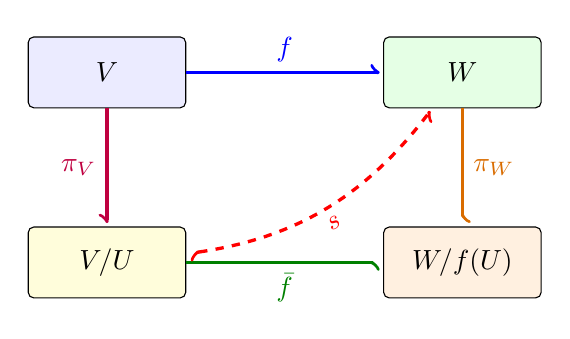
\begin{tikzpicture}[
  node distance=15mm and 25mm,
  object/.style={draw,rounded corners=2pt,minimum width=20mm,minimum height=9mm},
  map/.style={line width=1.2pt}
]
  \node[object,fill=blue!8] (V) {$V$};
  \node[object,fill=green!10,right=of V] (W) {$W$};
  \node[object,fill=yellow!14,below=of V] (Q) {$V/U$};
  \node[object,fill=orange!12,right=of Q] (R) {$W/f(U)$};

  \draw[map,blue,-{spaced left to}] (V) -- node[above] {$f$} (W);
  \draw[map,purple,-{spaced right to}] (V) -- node[left] {$\pi_V$} (Q);
  \draw[map,orange!85!black,-{spaced left to reversed}] (W) -- node[right] {$\pi_W$} (R);
  \draw[map,green!50!black,-{spaced right to reversed}] (Q) -- node[below] {$\bar f$} (R);
  \draw[map,dashed,red,{spaced left to reversed}-{spaced right to}]
    (Q) to[bend right=22] node[below,sloped] {$s$} (W);
\end{tikzpicture}
\end{document}
